\documentclass[12pt, twoside]{article}
\usepackage[letterpaper, margin=1in, headsep=0.5in]{geometry}
\usepackage[english]{babel}
\usepackage[utf8]{inputenc}
\usepackage{amsmath}
\usepackage{amsfonts}
\usepackage{amssymb}
\usepackage{tikz}
\usepackage{yhmath}
\usetikzlibrary{quotes, angles}
\usepackage{graphicx}
\usepackage{enumitem}
\usepackage{multicol}

\newif\ifmeta
\metatrue %print standards and topics tags

\title{Regents Geometry}
\author{Chris Huson}
\date{May 2022}

\usepackage{fancyhdr}
\pagestyle{fancy}
\fancyhf{}
\renewcommand{\headrulewidth}{0pt} % disable the underline of the header
\raggedbottom

\fancyhead[LE]{\thepage}
\fancyhead[RO]{\thepage \\ Name: \hspace{4cm} \,\\}
\fancyhead[LO]{BECA / Dr. Huson, Mr. Segal / Geometry\\* Unit 12: IB Trigonometry\\* 25 May 2022}

\begin{document}

\subsubsection*{12.3 Law of cosines \hfill HSG.SRT.D.11}
\textbf{Formulas}\\[0.25cm]
Cosine rule: $c^2=a^2+b^2-2ab \cos C$\\[0.25cm]
Sine rule: $\displaystyle \frac{a}{\sin A} = \frac{b}{\sin B}$\\[0.25cm]
Area of a right triangle: $\displaystyle A=\frac{1}{2}(bh)$, where $b$ is the base, $h$ is the height\\[0.25cm]
Area of any triangle: $\displaystyle A=\frac{1}{2}ab \sin C$

\begin{enumerate}
  \item The following diagram shows triangle $ABC$, with $BC=10$, $A\hat{C}B=28^\circ$, and $AC=8$ cm. \\[0.25cm]
  Find $AB$. \hfill \emph{diagram not to scale}
    \begin{flushright}
      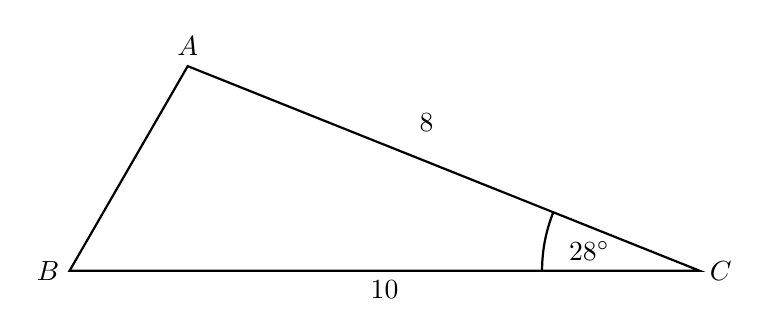
\begin{tikzpicture}[scale=1]
        \draw [thick](60:3)node[above]{$A$}--
        (0,0)node[left]{$B$}--
        (0:8)node[right]{$C$}--cycle;
        \node at (25:5)[below]{$8$};
        %\draw [thick, -] (0:1) arc [start angle=0, end angle=60, radius=1];
        \node at (0:4)[below]{$10$};
        \draw [thick, -] (0:6) arc [start angle=180, end angle=158, radius=2];
        \node at (0:6.6)[above]{$28^\circ$};
      \end{tikzpicture}
    \end{flushright}\vspace{2cm}
  
  \item Triangle $ABC$ has side lengths $AB=12.8$ and $BC=10.4$, while $A\hat{B}C=58^\circ$. \\[0.25cm]
  Find $AC$.
    \begin{flushright}
      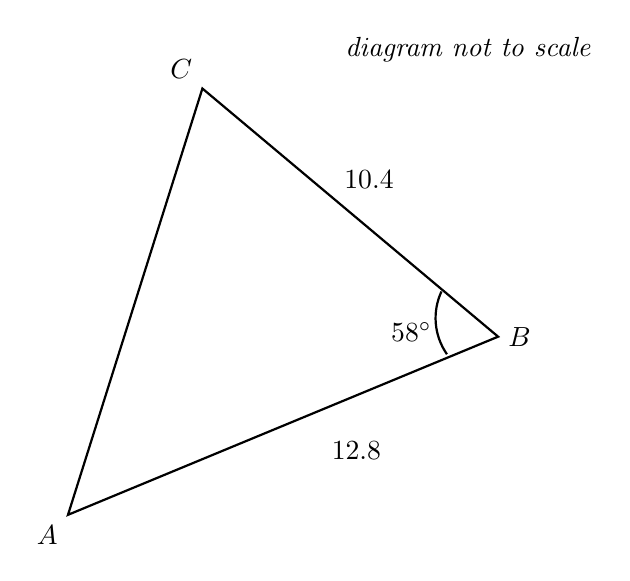
\begin{tikzpicture}[scale=0.8]
        %\draw [thick] (0,0) circle [radius=4];
        %\draw [dashed] (0,0)node[below]{$O$}--(100:4);
        \draw [thick](0:4)node[right]{$B$}--
        (100:4)node[above left]{$C$}--
        (-135:4)node[below left]{$A$}--cycle;
        \node at (55:3.4)[below]{$10.4$};
        \node at (1.75,-2.1)[above]{$12.8$};
        \draw [thick, -] (-5:3.2) arc [start angle=215, end angle=155, radius=1];
        \node at (1.5:3.1)[left]{$58^\circ$};
        \node at (50:5.5)[above]{\emph{diagram not to scale}};
      \end{tikzpicture}
    \end{flushright}
  
  \newpage
  \item The following diagram shows triangle $ABC$, with $A\hat{B}C=54^\circ$, $A\hat{C}B=33^\circ$, and $BC=10.8$. \\[0.25cm]
  (i) Write down $B\hat{A}C$
  (ii) Now find $AC$.\hfill \emph{diagram not to scale}
    \begin{flushright}
      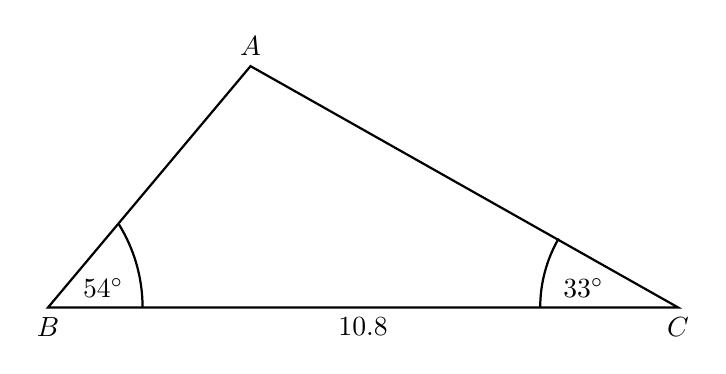
\begin{tikzpicture}[scale=1]
        \draw [thick](50:4)node[above]{$A$}--
        (0,0)node[below]{$B$}--
        (0:8)node[below]{$C$}--cycle;
        \node at (0:4)[below]{$10.8$};
        \draw [thick, -] (0:1.2) arc [start angle=0, end angle=32, radius=2];
        \node at (0:0.7)[above]{$54^\circ$};
        \draw [thick, -] (0:6.25) arc [start angle=180, end angle=150, radius=1.75];
        \node at (0:6.8)[above]{$33^\circ$};
      \end{tikzpicture}
    \end{flushright}\vspace{1cm}
  
  \item The following right-angled triangle $ABC$ has side lengths $AB=6.8$ and $BC=4.6$.
  \\[0.25cm]
  Find the area of the triangle. \hfill \emph{diagram not to scale}
    \begin{flushright}
      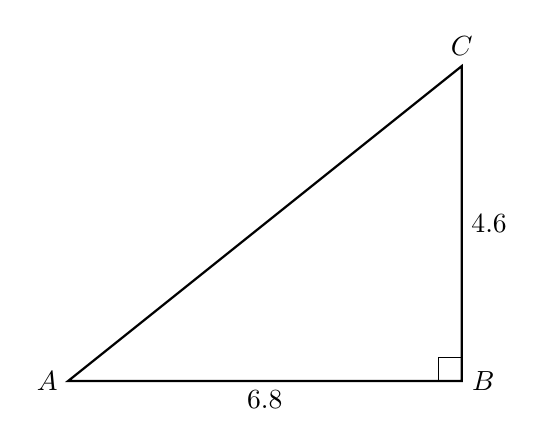
\begin{tikzpicture}[scale=1]
        \draw [thick](0,0)node[left]{$A$}--
        (5,0)node[right]{$B$}--
        (5,4)node[above]{$C$}--cycle;
        \node at (2.5,0)[below]{$6.8$};
        \node at (5,2)[right]{$4.6$};
        \draw (4.7,0)--++(0,0.3)--++(0.3,0);
      \end{tikzpicture}
    \end{flushright}\vspace{1cm}
  
  \item The following triangle $DEF$ has side lengths $DE=7$ and $EF=9$, with $D\hat{E}F=72^\circ$. 
  \\[0.25cm]
  Find the area of the triangle. \hfill \emph{diagram not to scale}
    \begin{flushright}
      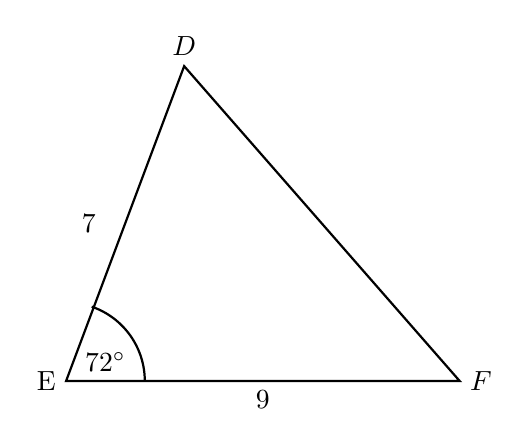
\begin{tikzpicture}[scale=1]
        \draw [thick](0,0)node[left]{E}--
        (5,0)node[right]{$F$}--
        (1.5,4)node[above]{$D$}--cycle;
        \node at (2.5,0)[below]{$9$};
        \node at (0.5,2)[left]{$7$};
        \node at (0.5,0)[above]{$72^\circ$};
        \draw [thick, -] (1,0) arc [start angle=0, end angle=71, radius=1];
      \end{tikzpicture}
    \end{flushright}\vspace{1cm}  

\end{enumerate}
\end{document}
  